\newpage
\section{Objetivos}

Ao longo de todas essas práticas, nosso objetivo é estudar o comportamento de ondas transversais estacionárias em cordas e em colunas de ar, e determinar a velocidade de propagação das ondas progressivas em cada um desses meios.\\

Para isso, realizaremos 5 experimentos envolvendo diferentes instrumentos, que serão explicados a seguir.\\

\begin{figure}[H]
  \centering
  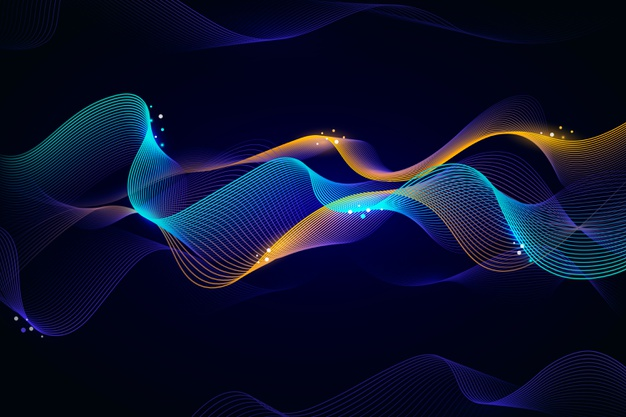
\includegraphics[scale=0.6]{images/waves1.jpg}
  \caption{Ondas}
\end{figure}
